\documentclass[a4paper]{report}
\usepackage[svgnames,dvipsnames,table,xcdraw]{xcolor}
\renewcommand{\textbf}[1]{\begingroup\bfseries\mathversion{bold}#1\endgroup}
%\usepackage[latin1]{inputenc}
\usepackage[french]{babel}
\usepackage[T1]{fontenc} 
%\usepackage[utf8]{inputenc}
\usepackage{textcomp}
\usepackage{graphicx,wrapfig,lipsum}

\usepackage{caption}
\usepackage{subcaption}
\usepackage{amsfonts}
\usepackage{amsmath}
\usepackage[left=2.5cm,right=2.5cm,top=2cm,bottom=3cm]{geometry}
\usepackage{tikz}
\usepackage{tikz-3dplot}
\usepackage{array}
\usepackage{tabularx}
\usepackage{glossaries}
\setlength{\doublerulesep}{\arrayrulewidth}

\usepackage{multicol}
\usepackage{marvosym}
\usepackage{amssymb}
\AddThinSpaceBeforeFootnotes
\FrenchFootnotes
\setlength\parindent{0pt}
\usepackage{cancel}
\usepackage{multicol}
\usepackage{enumitem}
%\usepackage{pifont}
\usepackage{marvosym}
\usepackage{comment}
\usepackage{fancyhdr}
\usepackage{xltxtra}
\setmainfont{Cambria}
\usepackage{listings}
\pagestyle{fancy}


\usepackage{minitoc}
\usepackage{titlepic}
\usepackage{datetime}

\rhead{Olivier Bützberger \& Bastien Vallat}
\lhead{\today}

\renewcommand\thesection{\arabic{section}}

\begin{document}

\begin{center}
\textbf{Biologie des populations, série 3}
\end{center}

\textbf{R1}\\
\textit{1)} La taille efficace $N_e$ d'une population peut se définir comme l'effectif que doit avoir une population idéale pour évoluer et dériver au même taux qu'observé dans la population réelle étudiée et dont la variance serait aussi perdue au même taux que dans cette population réelle étudiée. D'après le cours de Génétique des population de J.Goudet, une population idéale est "une population de taille finie\textit{(1)} ou les croisements sont aléatoires\textit{(2)}, les générations non recouvrantes\textit{(3)}, sans sélection\textit{(4)} ni migration\textit{(5)} ni mutation\textit{(6)}"(p.47). \\

\textit{2)} 
$N_e>N$ : On peut observer ce cas lorsque la dispersion est faible (par exemple si on considère plusieurs sous population entre lesquels il y a très peu de dispersion). En effet, cela va contribuer à conserver la variance génétique et donc, la dérive génétique sera faible (p.69-70 du cours).\\

$N_e<N$ :  Au contraire du cas présenté ci-dessus, si la dispersion est très grande et que la perte de variance de variance génétique est plus rapide que dans une population idéale, l'effectif efficace sera plus faible que l'effectif de la population idéale. Nous trouvons un exemple à la page 53 du cours avec le cas d'un sex-ratio biaisé qui va diminuer la taille efficace. Une population avec 10 mâles et 90 femelles aura une taille de 36 individus ($N_e=\frac{4N_mN_f}{N_m+N_f}$) alors que sa taille réelle est de 100 individus. La raison avancée est que dans ce cas là, "les mâles participent beaucoup plus à la reproduction que les femelles" (p.53).\\

\textbf{R2}\\
\textit{A)} Si la fréquence initiale est basse, la probabilité de fixation de l'allèle est faible (a). Alors que si la fréquence initiale est haute, la probabilité de fixation est également haute (b). 

\begin{figure}[!h]
	
	\begin{subfigure}{.5\textwidth}
		\centering
		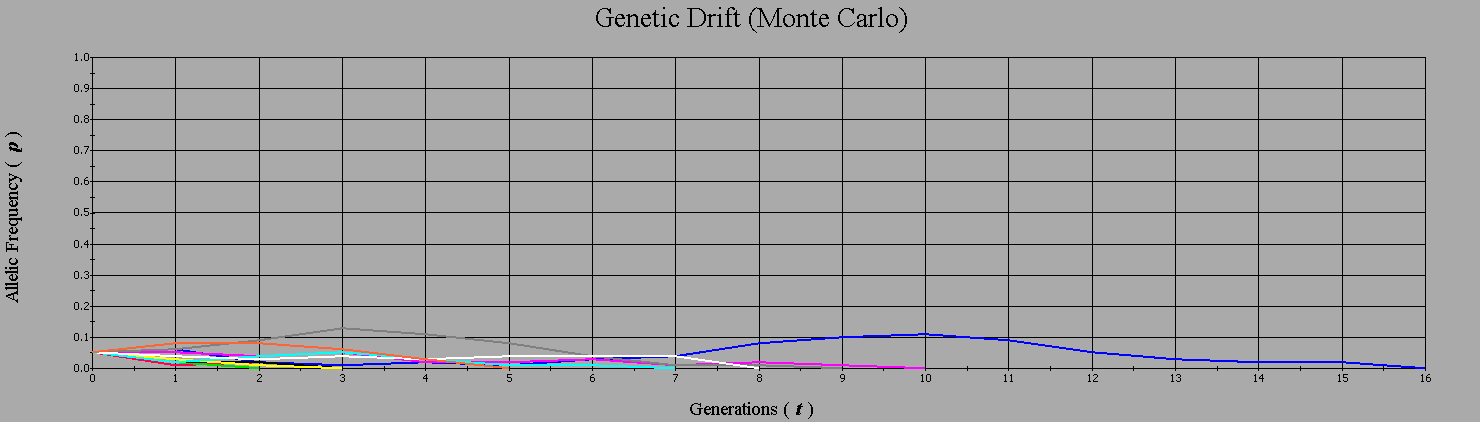
\includegraphics[width=.99\linewidth]{r2.png}
		\caption{Fréquence initiale : 0.05}
	\end{subfigure}%
	\begin{subfigure}{.5\textwidth}
		\centering
		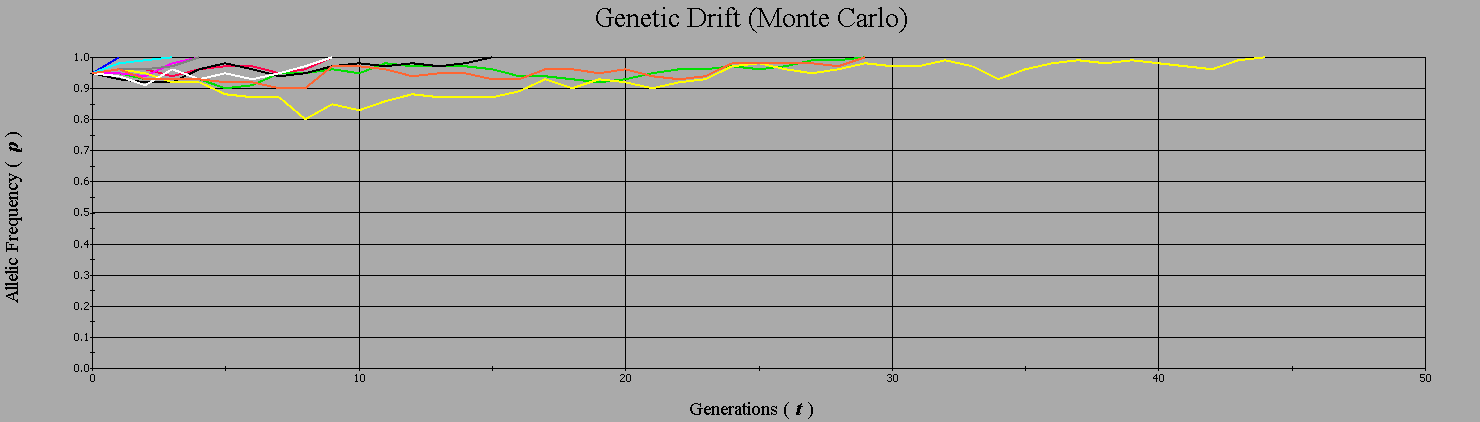
\includegraphics[width=.99\linewidth]{r2_2.png}
		\caption{Fréquence initiale : 0.95}
	\end{subfigure}\\


\textit{B)} Dans les figures ci-dessous, on voit que si la taille de la population est élevée, il faudra plus de temps pour observer la fixation ou la perte d'un allèle. Dans les 2 cas, la taille de la population n'affecte pas la probabilité de fixation. 


	\begin{subfigure}{.5\textwidth}
		\centering
		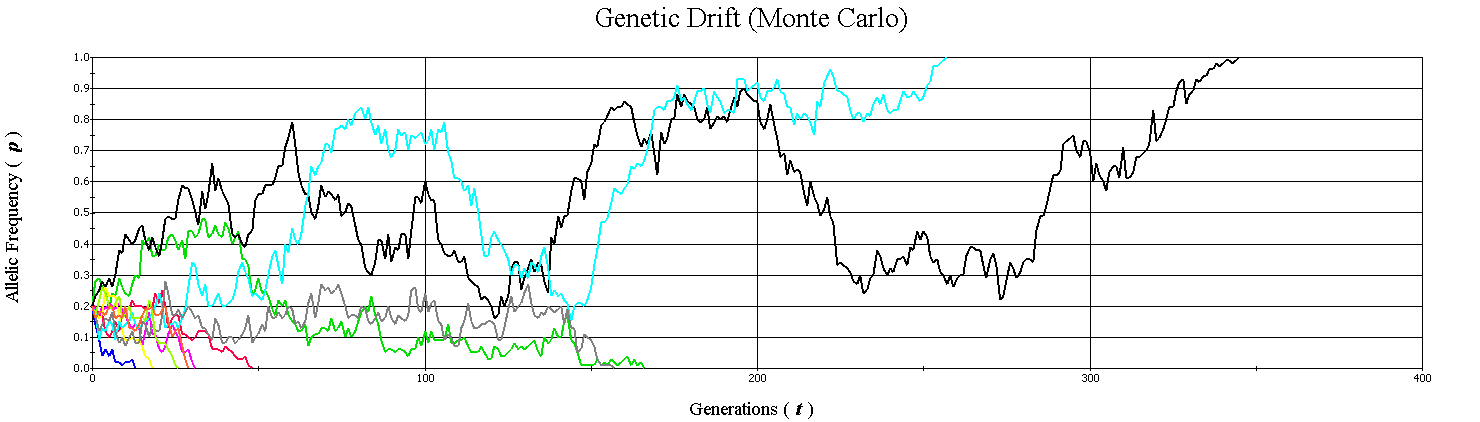
\includegraphics[width=.99\linewidth]{r3_1.png}
		\caption{N=50}
	\end{subfigure}%
	\begin{subfigure}{.5\textwidth}
		\centering
		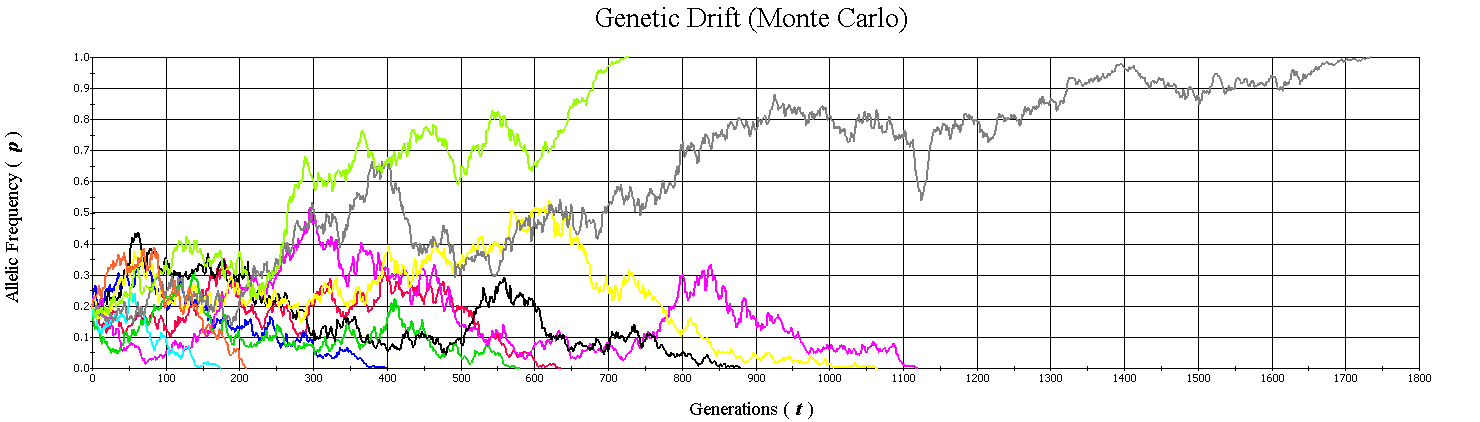
\includegraphics[width=.99\linewidth]{r3_2.png}
		\caption{N=500}
	\end{subfigure}


\textbf{R3}\\
\textit{A)}\\
$F_t$ = courbe théorique - coefficient de consanguinité théorique (indice de fixation)\\
$F_a$ = F observé dans la population. \\
$F_p$ = Autozygotie actuelle de la population entière.\\

\textit{B)}\\
	\begin{subfigure}{.5\textwidth}
	\centering
	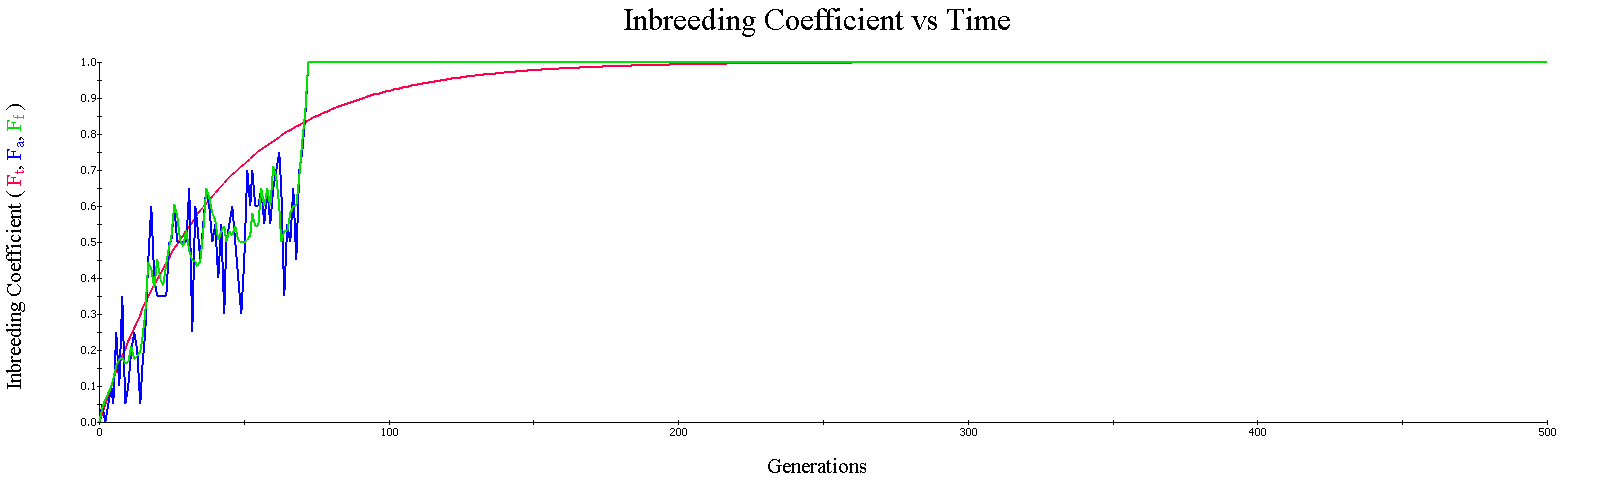
\includegraphics[width=.99\linewidth]{r3_3.png}
	\caption{Population = 20}
\end{subfigure}%
\begin{subfigure}{.5\textwidth}
	\centering
	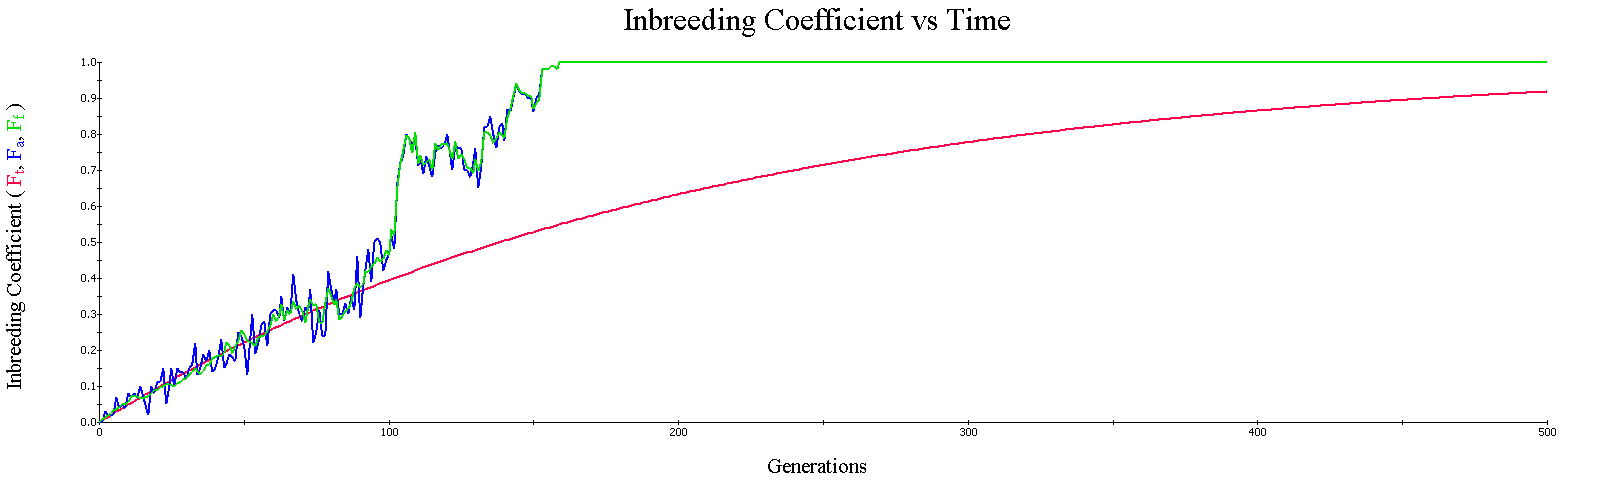
\includegraphics[width=.99\linewidth]{r3_4.png}
	\caption{Population = 200}
\end{subfigure}

\end{figure}
Dans la figure (e), avec une population de petite taille, l'indice de fixation théorique atteint très rapidement 1 (100\% d'homozygotes). Il n'y a plus qu'un seul allèle dans la population. La dérive est forte. Dans le cas où la population est de grande taille, la dérive génétique est plus faible et l'indice de fixation théorique met beaucoup plus de temps avant d'arriver à 1. 





















\end{document}